\section{Dwi Septiani Tsaniyah(1174003)}
\subsection{PYSHP Reader}
\begin{enumerate}
    \item Buatlah Script Python dan jelaskan berbaris
    \lstinputlisting[firstline=1, lastline=3]{src/1174003/3/praktikum3.py}
    \hfill\break
    \begin{figure}[H]
		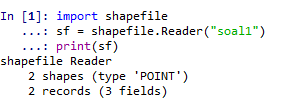
\includegraphics[width=4cm]{figures/1174003/3/1.png}
		\centering
		\caption{Hasil SHP Reader Soal 1}
    \end{figure}
    
    \item Buatlah Script Python dan jelaskan berbaris
    \lstinputlisting[firstline=5, lastline=7]{src/1174003/3/praktikum3.py}
    \hfill\break
    \begin{figure}[H]
		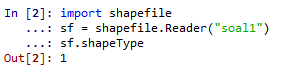
\includegraphics[width=4cm]{figures/1174003/3/2.png}
		\centering
		\caption{Hasil SHP Reader Soal 2}
    \end{figure}
    
    \item Buatlah Script Python dan jelaskan berbaris
    \lstinputlisting[firstline=9, lastline=11]{src/1174003/3/praktikum3.py}
    \hfill\break
    \begin{figure}[H]
		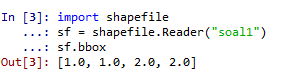
\includegraphics[width=4cm]{figures/1174003/3/3.png}
		\centering
		\caption{Hasil SHP Reader Soal 3}
    \end{figure}
    
    \item Buatlah Script Python dan jelaskan berbaris
    \lstinputlisting[firstline=13, lastline=16]{src/1174003/3/praktikum3.py}
    \hfill\break
    \begin{figure}[H]
		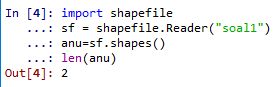
\includegraphics[width=4cm]{figures/1174003/3/4.png}
		\centering
		\caption{Hasil SHP Reader Soal 4}
    \end{figure}
    
    \item Buatlah Script Python dan jelaskan berbaris
    \lstinputlisting[firstline=18, lastline=22]{src/1174003/3/praktikum3.py}
    \hfill\break
    \begin{figure}[H]
		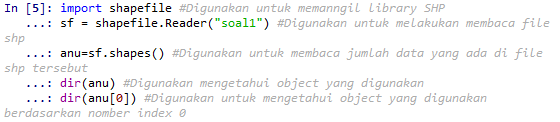
\includegraphics[width=4cm]{figures/1174003/3/5.png}
		\centering
		\caption{Hasil SHP Reader Soal 5 Codingan}
    \end{figure}

    \hfill\break
    \begin{figure}[H]
		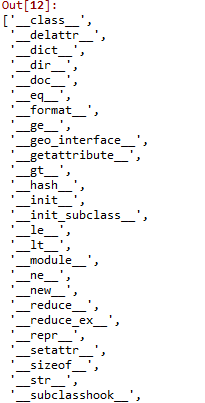
\includegraphics[width=4cm]{figures/1174003/3/5_out.png}
		\centering
		\caption{Hasil SHP Reader Soal 5 Hasil}
    \end{figure}
    
    \item Buatlah Script Python dan jelaskan berbaris
    \lstinputlisting[firstline=24, lastline=27]{src/1174003/3/praktikum3.py}
    \hfill\break
    \begin{figure}[H]
		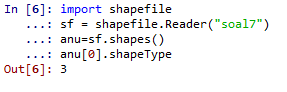
\includegraphics[width=4cm]{figures/1174003/3/6.png}
		\centering
		\caption{Hasil SHP Reader Soal 6}
    \end{figure}

    \item Buatlah Script Python dan jelaskan berbaris
    \lstinputlisting[firstline=29, lastline=32]{src/1174003/3/praktikum3.py}
    \hfill\break
    \begin{figure}[H]
		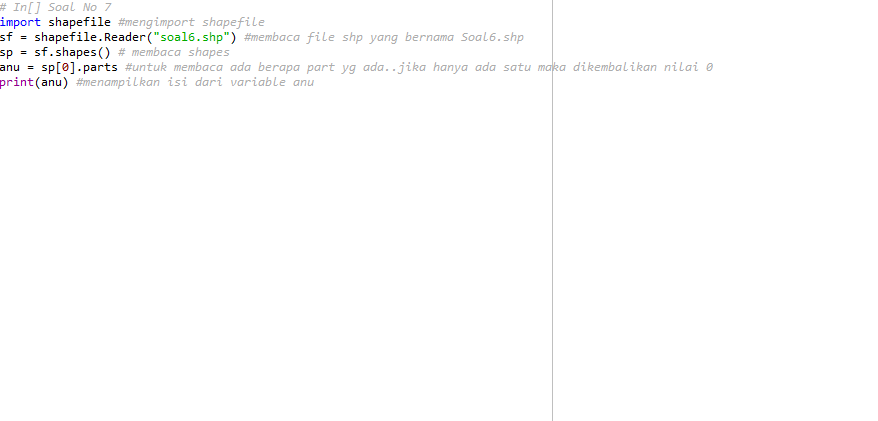
\includegraphics[width=4cm]{figures/1174003/3/7.png}
		\centering
		\caption{Hasil SHP Reader Soal 7}
    \end{figure}

    \item Buatlah Script Python dan jelaskan berbaris
    \lstinputlisting[firstline=37, lastline=40]{src/1174003/3/praktikum3.py}
    \hfill\break
    \begin{figure}[H]
		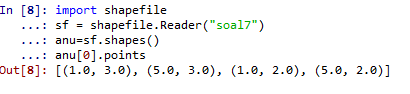
\includegraphics[width=4cm]{figures/1174003/3/8.png}
		\centering
		\caption{Hasil SHP Reader Soal 8}
    \end{figure}

    \item Buatlah Script Python dan jelaskan berbaris
    \lstinputlisting[firstline=42, lastline=45]{src/1174003/3/praktikum3.py}
    \hfill\break
    \begin{figure}[H]
		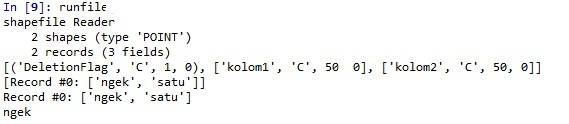
\includegraphics[width=4cm]{figures/1174003/3/9.jpg}
		\centering
		\caption{Hasil SHP Reader Soal 9}
    \end{figure}

    \item Buatlah Script Python dan jelaskan berbaris
    \lstinputlisting[firstline=47, lastline=50]{src/1174003/3/praktikum3.py}
    \hfill\break
    \begin{figure}[H]
		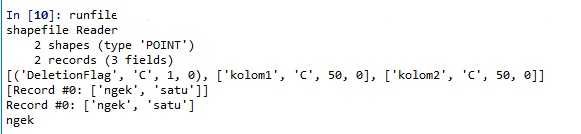
\includegraphics[width=4cm]{figures/1174003/3/10.jpg}
		\centering
		\caption{Hasil SHP Reader Soal 10}
    \end{figure}

    \item Buatlah Script Python dan jelaskan berbaris
    \item \lstinputlisting[firstline=52, lastline=56]{src/1174003/3/praktikum3.py}
    \hfill\break
    \begin{figure}[H]
		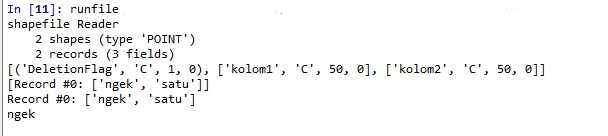
\includegraphics[width=4cm]{figures/1174003/3/11.jpg}
		\centering
		\caption{Hasil SHP Reader Soal 11}
    \end{figure}
\end{enumerate}
\subsection{Link Youtube}
\href{https://youtu.be/Apvppjotft8}{Video Youtube}